%%%%%%%% 18-789 Final Project Report (course submission, non-anonymous) %%%%%%%%%%%%%%%%%
% Build: make report (see Makefile and README.md)

\documentclass{article}

\usepackage{microtype}
\usepackage{graphicx}
\usepackage{booktabs}
\usepackage{array}
\usepackage{amsmath,amssymb}
\usepackage{tikz}
\usetikzlibrary{positioning,arrows.meta,fit}
\usepackage{hyperref}
\usepackage{subcaption}
\newcommand{\theHalgorithm}{\arabic{algorithm}}
\usepackage[accepted]{reportstyle}

% All three authors share the same affiliation, so the "^1" superscripts add
% no information. Suppress the per-author superscript and drop the leading
% "^1" in the affiliation footnote, while still registering the affiliation
% counter so the institution string is printed.
\makeatletter
\renewcommand\@pa[1]{%
  \ifcsname the@affil#1\endcsname\else
    \stepcounter{@affiliationcounter}%
    \newcounter{@affil#1}%
    \setcounter{@affil#1}{\value{@affiliationcounter}}%
  \fi
}
\renewcommand{\printAffiliationsAndNotice}[1]{%
\stepcounter{@affiliationcounter}%
{\let\thefootnote\relax\footnotetext{\hspace*{-\footnotesep}\ifdefined\isaccepted #1\fi%
\forloop{@affilnum}{1}{\value{@affilnum} < \value{@affiliationcounter}}{%
\ifcsname @affilname\the@affilnum\endcsname%
\csname @affilname\the@affilnum\endcsname%
\else
{\bf AUTHORERR: Missing \textbackslash{}reportaffiliation.}%
\fi
}.
\ifdefined\reportcorrespondingauthor@text
Correspondence to: \reportcorrespondingauthor@text.
\else
{\bf AUTHORERR: Missing \textbackslash{}reportcorrespondingauthor.}
\fi

\ \\
\Notice@String
}}}
\makeatother

\graphicspath{{figures/}{./}}

\reporttitlerunning{Diffusion Drafters for Speculative Speculative Decoding}

\begin{document}

\twocolumn[
\reporttitle{Diffusion Drafters for Speculative Speculative Decoding: When Parallel Drafting Fails to Beat Autoregression}

\begin{reportauthorlist}
\reportauthor{Aditya Ramesh}{cmu}
\reportauthor{Arav Tewari}{cmu}
\reportauthor{Xinyu Jiang}{cmu}
\end{reportauthorlist}

\reportaffiliation{cmu}{18-789 Final Project, Carnegie Mellon University, Pittsburgh, PA, USA}

\reportcorrespondingauthor{Xinyu Jiang}{xinyuj2@andrew.cmu.edu}

\reportkeywords{speculative decoding, LLM serving, diffusion language models, systems-ML}

\vskip 0.3in
]

\begin{abstract}
Speculative decoding (SD) accelerates LLM serving with a small draft model whose proposals a larger verifier accepts or rejects in one forward pass; speculative speculative decoding (SSD) pushes this further by pre-drafting the next window \emph{in parallel} with the verifier's current step, so draft latency is hidden behind the already-expensive verifier forward.
Because SSD's benefit scales with how much draft latency can be hidden, a natural hypothesis is that \emph{diffusion} drafters---which decode multiple tokens in one pass---should be especially good SSD partners.
We test this hypothesis on Qwen3-8B with three drafter families integrated into a single async SSD runtime: an autoregressive (AR) drafter, the one-pass block-diffusion drafter DFlash~\citep{dflash2025}, and the tree-structured diffusion drafter DDTree~\citep{ringel2026ddtree}.
Across batch sizes $b\in\{1,2,4\}$ and two output-length regimes (32 and 128), we evaluate three modes per family: \emph{exact-off} (SD-style synchronous drafting), \emph{exact-on oracle} (SSD with a perfect predictor---the architectural ceiling), and \emph{realized} (the actual asynchronous system).
The empirical story is a clean negative result: AR's oracle ceiling beats both diffusion oracles at every batch size in the main regime (up to $242$~tok/s at $b{=}4$ vs.\ $119$ and $141$ for DFlash and DDTree), and realized DFlash drops to ${\sim}9\%$ cache-hit rate and $24$--$36$~tok/s, well below its own SD baseline.
We trace this to a systems insight that contradicts the SSD paper's ``strictly faster than SD'' corollary in practice: SSD only helps when the drafter has \emph{serial} latency to hide, which diffusion drafters already removed.
\end{abstract}

%====================================================================
\section{Introduction / Motivation}
\label{sec:intro}

Autoregressive (AR) LLM decoding is fundamentally sequential: each token depends on the full prefix, so a 32B-parameter model pays a full forward pass per output token.
Speculative decoding (SD)~\citep{leviathan2023specdec,chen2023specsampling} breaks this by running a small \emph{draft} model to propose $k$ candidate tokens and then verifying them with one target-model forward; accepted tokens cost one verifier step, not $k$.
\emph{Speculative speculative decoding} (SSD)~\citep{kumar2026ssd} extends this by observing that while the verifier is computing step $t$'s logits, the drafter is idle---so the drafter can pre-speculate step $t{+}1$ by enumerating likely \emph{verification outcomes} (how many tokens get accepted, which bonus token is sampled) and pre-computing a speculation for each, overlapping future draft work with current verification.
The SSD paper proves a corollary (``strictly faster than SD'') that SSD with primary and backup speculators both set to $\mathcal{M}$ does no worse than SD with $\mathcal{M}$, assuming any positive cache-hit probability and zero overhead.

\paragraph{Problem statement.}
The SSD speedup depends on two things: (i)~how much \emph{sequential} drafter latency is available to hide, and (ii)~how well the drafter can predict the future prefix cheaply.
Current SSD systems assume an AR drafter.
\emph{Diffusion} language models~\citep{arriola2024blockdiffusion}, and in particular block-diffusion drafters such as DFlash~\citep{dflash2025}, generate an entire block of tokens in one parallel pass and are therefore faster per draft, but also force a different notion of ``future prefix.''
This sets up the core question of our project: can diffusion drafters---which parallelize \emph{within} a draft step---serve as better SSD drafters than AR drafters, given that SSD's whole purpose is to parallelize \emph{between} draft and verify steps?

\paragraph{Why this matters.}
LLM serving economics are dominated by decode-time throughput per GPU.
SD already gives $2$--$3{\times}$ throughput on practical verifiers; SSD promises another ${\sim}30$--$40\%$ on top.
If diffusion drafters compose well with SSD, they could give a multiplicative win and replace AR drafters across the stack.
If they do not---as this report finds---the community should stop treating ``more parallel drafter'' as axiomatically better for SSD, and instead measure \emph{where the hidden latency actually is}.

\paragraph{Goal and contributions.}
\textbf{(i)~An async drafter--verifier runtime} with pluggable speculator backends---we integrate AR (Qwen3-$\{0.6,1.7,4\}$B), DFlash~\citep{dflash2025}, and DDTree~\citep{ringel2026ddtree} drafters behind a common interface against a Qwen3-8B verifier~\citep{yang2024qwen3}; to our knowledge this is the first matched-budget comparison of these three drafter families under SSD.
\textbf{(ii)~A three-mode evaluation protocol} (exact-off / exact-on oracle / realized) that attributes gains or losses to \emph{architecture} vs.\ \emph{implementation} (\S\ref{ssec:modes}).
\textbf{(iii)~A negative empirical result with a mechanistic explanation}: under SSD, AR oracle $>$ diffusion oracle at every batch size in the main regime; realized diffusion drafters lose ${\sim}85$--$91\%$ of their SSD cache-hit headroom; the cause is that SSD's overlap has room to operate only when the drafter has serial latency to hide, which diffusion drafters already removed.

%====================================================================
\section{Background and Related Work}
\label{sec:related}

\subsection{Background: SD, SSD, and diffusion drafters}
\label{ssec:bg}

\paragraph{Speculative decoding (SD)~\citep{leviathan2023specdec,chen2023specsampling}.}
A small drafter $\mathcal{M}_d$ proposes $k$ candidate tokens from prefix $x_{1:t}$; the verifier $\mathcal{M}_v$ scores all $k$ in \emph{one} forward, and rejection sampling on $p_v/p_d$ yields the longest accepted prefix plus a bonus verifier token---an exactness-preserving $1{+}\text{accepted}$ tokens per verifier step.
Throughput improves whenever $\mathcal{M}_d$ is much cheaper than $\mathcal{M}_v$ \emph{and} the accept rate is high.

\paragraph{Speculative speculative decoding (SSD)~\citep{kumar2026ssd}.}
While the verifier processes round $T$, a \emph{primary} speculator predicts a small set of likely \emph{verification outcomes} $v\,{=}\,(k,t^*)$ from its own logits (number of accepted tokens $k$ and bonus token $t^*$), pre-speculates a continuation for each in parallel, and stores them in a \emph{speculation cache} indexed by outcome.
On a hit the cached speculation is returned for free; on a miss, a \emph{backup} speculator runs the synchronous fallback.
SSD's Corollary~8 (``strictly faster than SD'') guarantees $\mathrm{SSD}\succeq\mathrm{SD}$ with both speculators set to $\mathcal{M}$, $p_{\text{hit}}{>}0$, and zero overhead---an assumption we challenge in~\S\ref{sec:disc}.

\paragraph{DFlash~\citep{dflash2025}.}
A one-pass \emph{block-diffusion} drafter: given prefix $x_{1:t}$, it predicts a block $\hat{x}_{t:t+B}$ in a \emph{single} masked-diffusion forward (input is prefix $\|$ $B$~\texttt{[MASK]}; KV cache injected into prefix attention).
Trades per-token quality for ${\sim}10{\times}$ lower per-block latency, which makes it an attractive SSD drafter candidate.

\paragraph{DDTree~\citep{ringel2026ddtree}.}
From the per-position marginals of one DFlash forward, a best-first heap selects up to $N$ tree nodes maximizing the drafter's factorized expected-acceptance surrogate (a block-diffusion adaptation of OPT-Tree); the tree is verified in one batched target forward with ancestor-only attention---closer in spirit to SpecInfer~\citep{miao2024specinfer} than to AR tree drafters.
We use DDTree as released and integrate it---together with AR and DFlash---into our async SSD runtime.

\subsection{Related work}

\paragraph{Synchronous SD families.}
Tree variants (SpecInfer~\citep{miao2024specinfer}, Medusa~\citep{cai2024medusa}) draft multiple branches to raise accept rate; EAGLE~\citep{li2024eagle} replaces the drafter with a feature-level head on the verifier.
All remain synchronous: verifier \emph{waits} for drafter.

\paragraph{Asynchronous / overlapped drafting.}
SSD~\citep{kumar2026ssd} is the most direct prior work.
TiDAR~\citep{tidar2025} and ``Your LLM Knows the Future''~\citep{sun2024ytllmfuture} use the target model itself to pre-speculate, which is more expensive but needs no separate drafter; we sit on the small-drafter side.
Block-diffusion~\citep{arriola2024blockdiffusion} and DFlash~\citep{dflash2025} are the closest prior diffusion drafters but were evaluated only under standard SD.

\paragraph{How our method differs.}
Prior work either measures drafters under SD alone, or evaluates SSD only with AR drafters.
We hold the drafter family variable \emph{and} sweep the three-mode protocol, so we can disentangle ``architecture is weak for SSD'' from ``implementation is weak for SSD'' on the same matched budget.

%====================================================================
\section{Methodology}
\label{sec:method}

\subsection{Why the method is non-trivial}
A naive ``plug diffusion in as the SSD drafter'' comparison is misleading for two reasons.
First, SSD's cache-hit rate depends on how well a \emph{future prefix} can be predicted cheaply, and diffusion drafters expose a fundamentally different future-state object than AR drafters do (a parallel block vs.\ a token sequence), so any evaluation must control for prediction quality separately from architecture.
Second, branch templates and tree budgets can be tuned per family and create an unfair advantage; we therefore fix a single branch template (\texttt{baseline48}) for all families and sweep only the knobs each method already exposes ($k$ for SD, $N$ for DDTree, $F$ for SSD).

\subsection{System overview}
Figure~\ref{fig:sys} shows the async runtime: a scheduler dispatches verify work on Qwen3-8B while a separate async speculator pre-computes speculations for a fanned-out set of likely verification outcomes, indexed by outcome in a speculation cache.
On a cache hit the pre-computed block is reused; on a miss the realized system falls back to a synchronous draft.
All three drafter families share one interface, which lets us hold scheduling, batching, and KV management constant across families.
At the algorithm level: SD runs \emph{Speculate}~$\to$~\emph{Verify}~$\to$~\emph{Speculate} sequentially; SSD pre-speculates $t{+}1$ in parallel with the $t$-th verify, harvesting savings only on successful prediction.

\begin{figure*}[t]
  \centering
  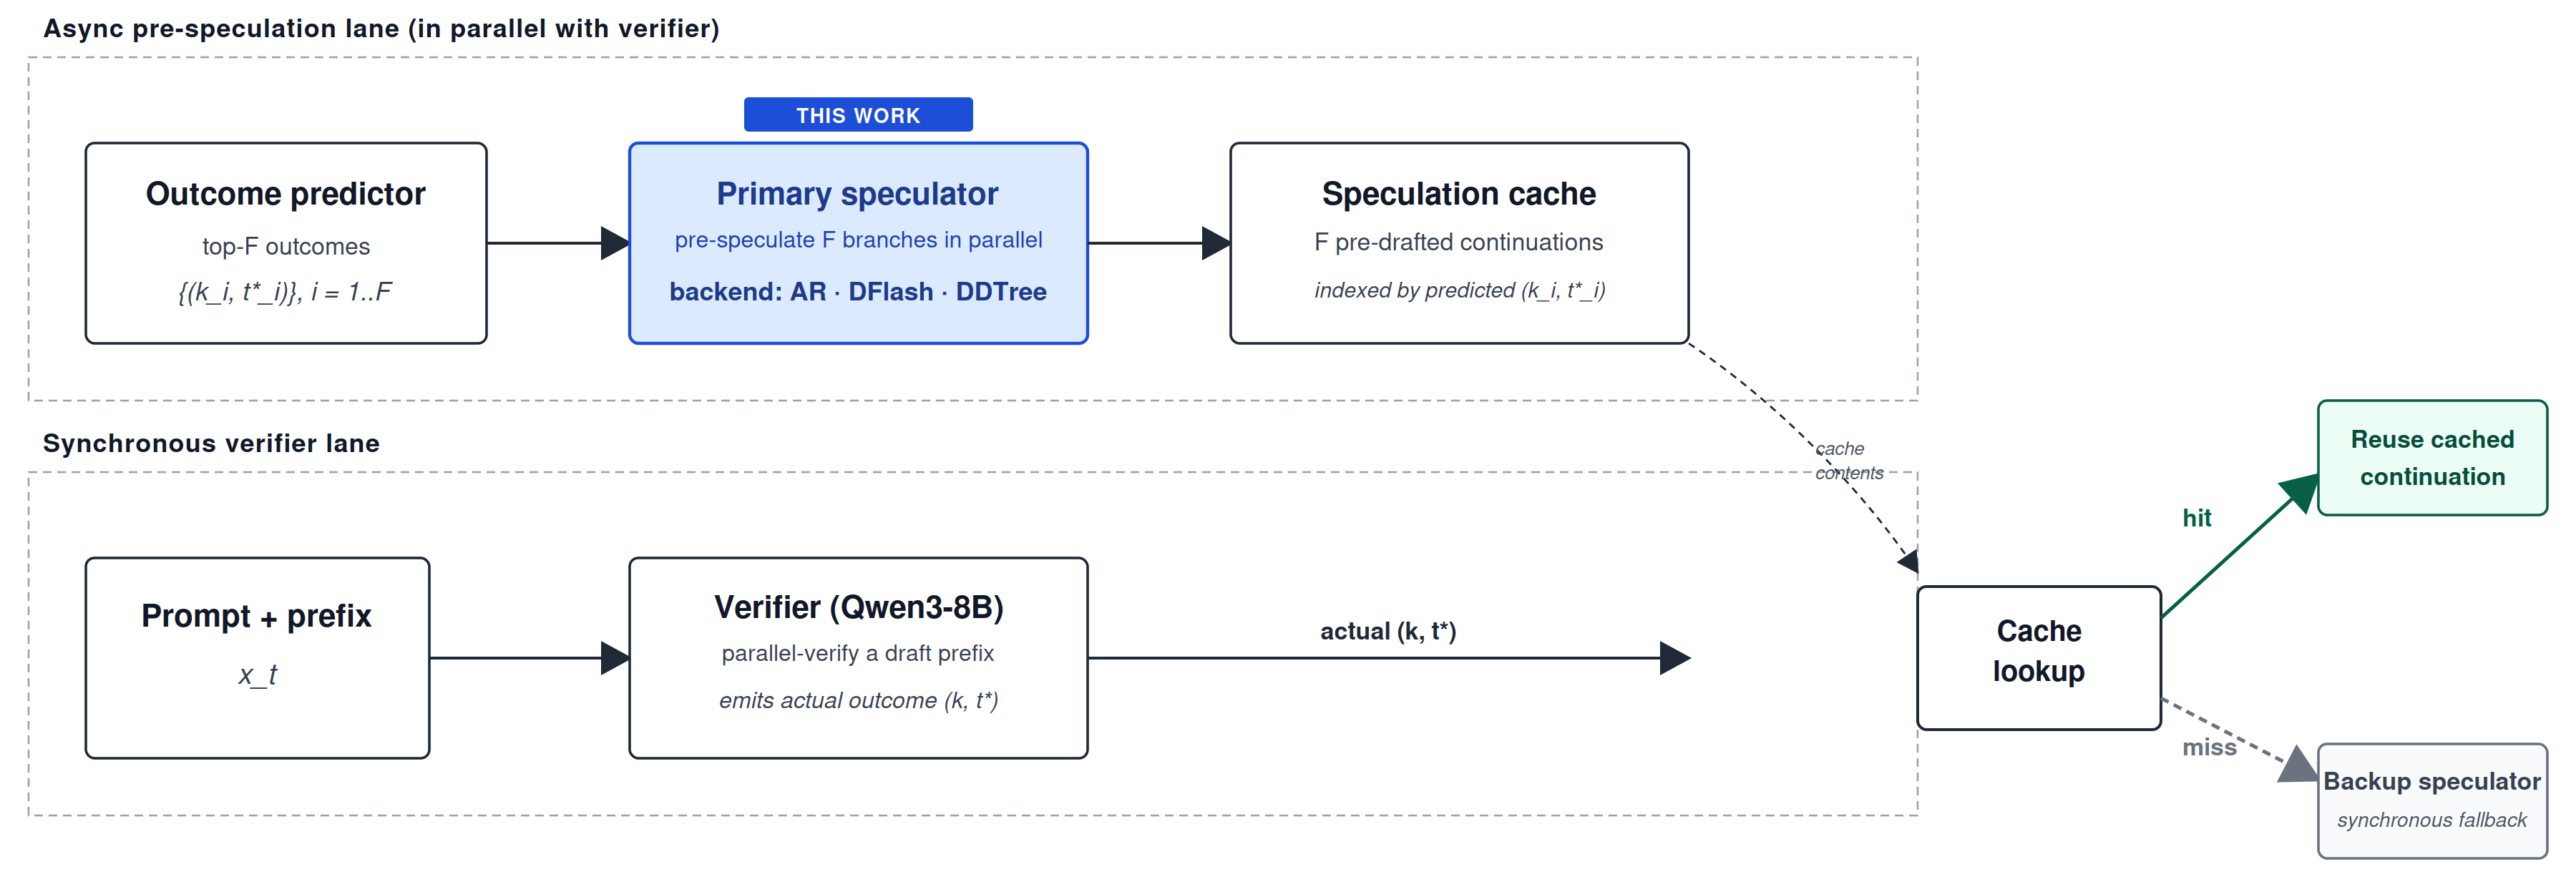
\includegraphics[width=0.96\textwidth]{fig01_async_ssd_runtime.png}
  \caption{Async SSD runtime with a pluggable speculator backend (SSD architecture from \citet{kumar2026ssd}).
  The async pre-speculation lane (top) issues top-$F$ predicted verification outcomes $\{(k_i,t^*_i)\}$ to the primary speculator, which pre-drafts a continuation for each into the speculation cache.
  The verifier lane (bottom) runs in parallel; once verification of step~$t$ emits the actual outcome $(k,t^*)$, the cache is queried.
  A hit reuses the matching pre-drafted continuation; a miss falls back to a synchronous backup speculator.
  In this work we vary only the speculator backend (\textbf{AR}, \textbf{DFlash}, \textbf{DDTree}); the runtime, predictor, cache, and verifier are held constant.}
  \label{fig:sys}
\end{figure*}

\subsection{Three evaluation modes (fairness gate)}
\label{ssec:modes}
For each drafter family we run three modes on the same prompts, verifier, and hardware:
\begin{description}
  \item[Exact-off.] Synchronous drafting; no SSD overlap. Baseline quality/speed of the drafter family (equivalent to standard SD).
  \item[Exact-on oracle.] SSD with a \emph{perfect} outcome predictor: the scheduler is given the realized verification outcome from the future, so the speculation cache always hits. The architectural ceiling---the best SSD could ever do for this family.
  \item[Realized.] The actual async system with a \emph{learned} predictor; cache hits are not guaranteed. The number a user would see in production.
\end{description}
Separating oracle from realized is crucial: if a family's oracle is not meaningfully above its exact-off, no amount of better prediction can save it (e.g.\ DFlash at $b{=}1$).

\subsection{Drafter families}
\label{ssec:families}
All three families are prior work; the matched-budget integration is ours.
\textbf{AR:} Qwen3-$\{0.6,1.7,4\}$B; token-by-token block of length $k$.
\textbf{DFlash}~\citep{dflash2025}: \texttt{z-lab/Qwen3-8B-DFlash-b16}, one-pass $b{=}16$ masked decode with KV injection.
\textbf{DDTree}~\citep{ringel2026ddtree}: tree-construction front-end on DFlash; we sweep DDTree's tree-node budget $N\in\{8,16\}$ jointly with SSD's outcome fan-out $F\in\{1,2\}$, and the verifier scores the tree in one batched forward with tree (ancestor-only) attention.
We fix the branch template (\texttt{baseline48}) across all families.

\subsection{DFlash predictor training}
Public DFlash checkpoints only support small verifiers, so we attempted to train a Qwen3-8B variant (KV injection, random masked-block sampling, loss weighting, shared embedding/LM head); the model exhibited \emph{mode collapse} (persistently predicting ``\textbackslash n\textbackslash n''), and neither removing KL distillation nor longer training resolved it within budget, so we fall back to the public DFlash-b16 checkpoint for all reported numbers.

%====================================================================
\section{Experimental Results}
\label{sec:exp}

\paragraph{Hardware and software.}
Target: Qwen3-8B.
Hardware: $2{\times}$H100 from Modal.
Decode: greedy.
Main regime: output length $32$, $b\in\{1,2,4\}$.
Extra SSD-favorable regime: output length $128$, same batch sizes.
Held-out: 78 prompt groups from our diffusion-drafter prompt split.
The drafter-scaling cross-check uses Qwen3-$\{0.6,1.7,4\}$B drafters against a Qwen3-32B verifier on GSM8K~\citep{cobbe2021gsm8k}.

\paragraph{Metrics.}
Decode throughput (tok/s); accepted suffix length per step; SSD cache hit rate; and---for the fairness gate---oracle vs.\ exact-off ratio (architectural headroom) and realized vs.\ oracle gap (predictor quality).
$95\%$ bootstrap confidence intervals are computed over prompt groups; error bars in all figures use this protocol.

\subsection{Drafter-scale cross-check (Qwen3-32B verifier)}
\label{ssec:scale}

\begin{table}[t]
  \caption{Cross-check on Qwen3-32B verifier, $b{=}1$, $k{=}4$, GSM8K: decode throughput (tok/s) as AR drafter size scales.
  \emph{AR} is target-only autoregressive decoding; \emph{SD} adds the AR drafter; \emph{SSD} adds SSD overlap on top.}
  \label{tab:ar-scale}
  \begin{center}
    \begin{small}
      \begin{tabular}{@{}lrrr@{}}
        \toprule
        Drafter      & AR  & SD  & SSD \\
        \midrule
        Qwen3-0.6B   & 94  & 161 & 186 \\
        Qwen3-1.7B   & 94  & 143 & 158 \\
        Qwen3-4B     & 94  & 106 &  99 \\
        \bottomrule
      \end{tabular}
    \end{small}
  \end{center}
\end{table}

We first orient on the drafter-scale axis (Table~\ref{tab:ar-scale}).
Smaller AR drafters are better SD partners ($186$~tok/s with the $0.6$B drafter vs.\ $99$~tok/s with the $4$B drafter)---the standard SD sweet-spot pattern.
The interesting row is the $4$B one: \emph{SSD$<$SD} ($99 < 106$).
When the drafter's per-call cost approaches the verifier's, SSD's free overlap has nothing to hide behind, and its scheduling overhead (CUDA streams, KV bookkeeping, wasted pre-draft on a miss) tips the inequality the wrong way.
The same mechanism will dominate the diffusion drafters in~\S\ref{ssec:oracle}---they are also ``too fat'' per call relative to the latency they leave to hide.

\subsection{Main result: oracle ceiling favors AR}
\label{ssec:oracle}

\begin{table}[t]
  \caption{Main regime (output length 32, $2{\times}$H100, Qwen3-8B verifier, greedy decode) by family and mode.
  \emph{Exact-off} is the same drafter under standard SD (no overlap); \emph{Oracle} is the SSD architectural ceiling; \emph{Realized} is the actual async system.}
  \label{tab:main}
  \begin{center}
    \begin{small}
      \setlength{\tabcolsep}{4pt}
      \begin{tabular}{@{}lrrrrr@{}}
        \toprule
        Family & $b$ & Exact-off & Oracle & Realized & Hit\% (real.) \\
        \midrule
        AR      & 1 &  40.1 &  79.9 &  63.6 & 60 \\
        AR      & 2 &  72.7 & 201.5 & 154.4 & 63 \\
        AR      & 4 & 125.5 & 242.1 & 125.4 & 57 \\
        \midrule
        DFlash  & 1 &  62.5 &  50.9 &  24.1 &  9 \\
        DFlash  & 2 &  95.6 &  91.8 &  30.1 &  9 \\
        DFlash  & 4 & 130.0 & 119.3 &  35.5 &  9 \\
        \midrule
        DDTree  & 1 &  82.0 &  81.5 &  67.9 &  $<$1 \\
        DDTree  & 2 & 125.0 & 119.3 &  97.2 &  $<$1 \\
        DDTree  & 4 & 157.8 & 141.1 & 131.4 &  $<$1 \\
        \bottomrule
      \end{tabular}
    \end{small}
  \end{center}
\end{table}

Table~\ref{tab:main} answers our central question.
The AR oracle reaches $242$~tok/s at $b{=}4$, while DFlash and DDTree oracles reach only $119$ and $141$~tok/s respectively, even though the diffusion families decode multiple tokens in parallel per draft.
DDTree is the strongest diffusion family but only ties AR at $b{=}1$ ($81.5$ vs.\ $79.9$); it falls behind from $b{=}2$ onward.
In the extra regime (output length~$128$, summarized in~\S\ref{ssec:extra}) DDTree oracle exceeds AR at $b{=}1$ ($128$ vs.\ $106$) but AR recovers the lead from $b{=}4$ onward---the upside is narrow and regime-specific.
Critically, observe the \emph{exact-off} column: for DFlash and DDTree, oracle is \emph{at or below} exact-off, meaning that even a perfect predictor cannot help these families.

\begin{figure*}[t]
  \centering
  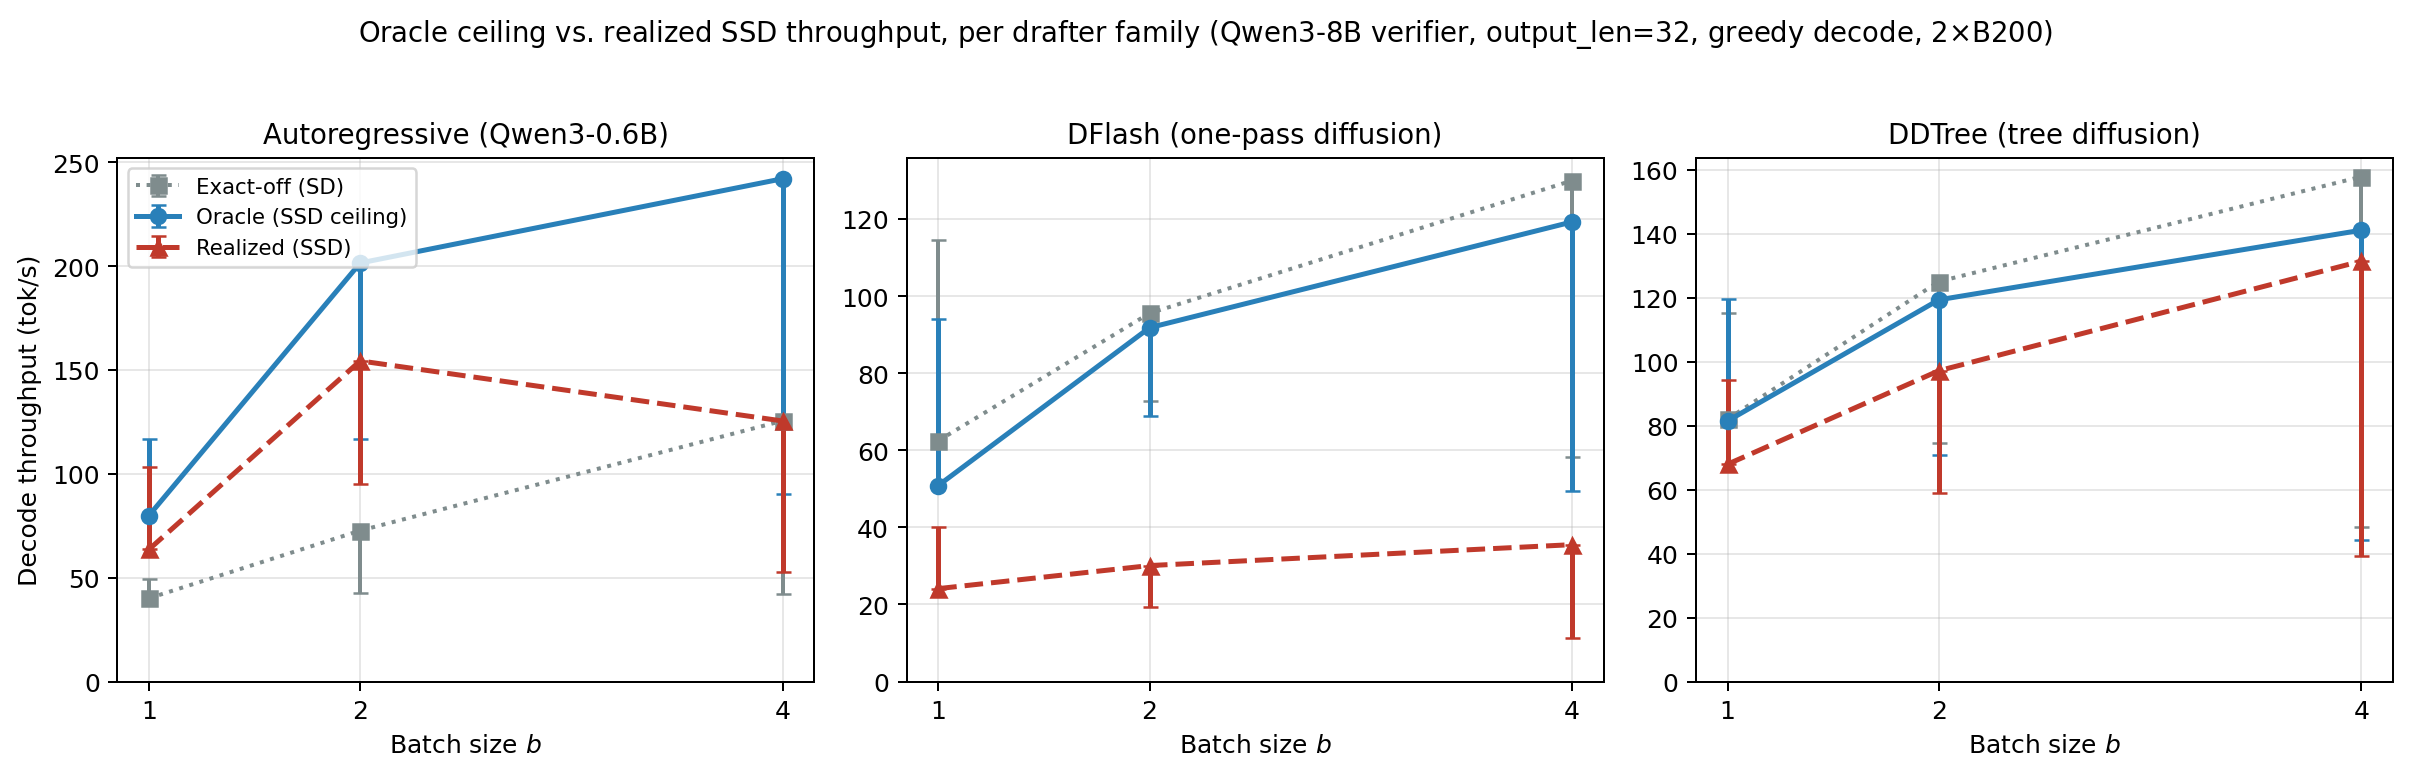
\includegraphics[width=0.96\textwidth]{fig09b_oracle_vs_realized_per_family.png}
  \caption{Per-family decomposition of oracle vs.\ realized vs.\ exact-off SD throughput (held constant: Qwen3-8B verifier, output length~$32$, greedy decode, $2{\times}$H100, fixed branch template \texttt{baseline48}; error bars are $95\%$ bootstrap CIs over prompt groups).
  \textbf{AR (left):} large gap between oracle and exact-off (${\sim}2{\times}$ headroom), realized still beats SD.
  \textbf{DFlash (middle):} oracle sits \emph{below} exact-off for all $b$; realized collapses to ${\sim}30\%$ of SD because the predictor cache-hit rate is only $9\%$.
  \textbf{DDTree (right):} oracle barely matches exact-off; realized loses more than half its hit headroom.}
  \label{fig:per-family}
\end{figure*}

Figure~\ref{fig:per-family} visualizes Table~\ref{tab:main} with one panel per family, on the same axes for each panel; this is the cleanest single picture of the whole project.
Reading the panels left-to-right, the AR drafter shows the pattern SSD was designed for---a large oracle gap above exact-off, with the realized system capturing more than half of it at every batch size.
DFlash shows the failure mode: the oracle line is at or below the exact-off line for all batch sizes, so the SSD architecture has no room to operate, and the realized line collapses underneath both.
DDTree sits in between but tells the same story---the oracle barely peeks above exact-off at $b{=}1$ and dips below for $b{\ge}2$, so the realized system is at best a small step down from exact-off.

\subsection{Architectural headroom: oracle / exact-off}
\label{ssec:headroom}

\begin{figure*}[t]
  \centering
  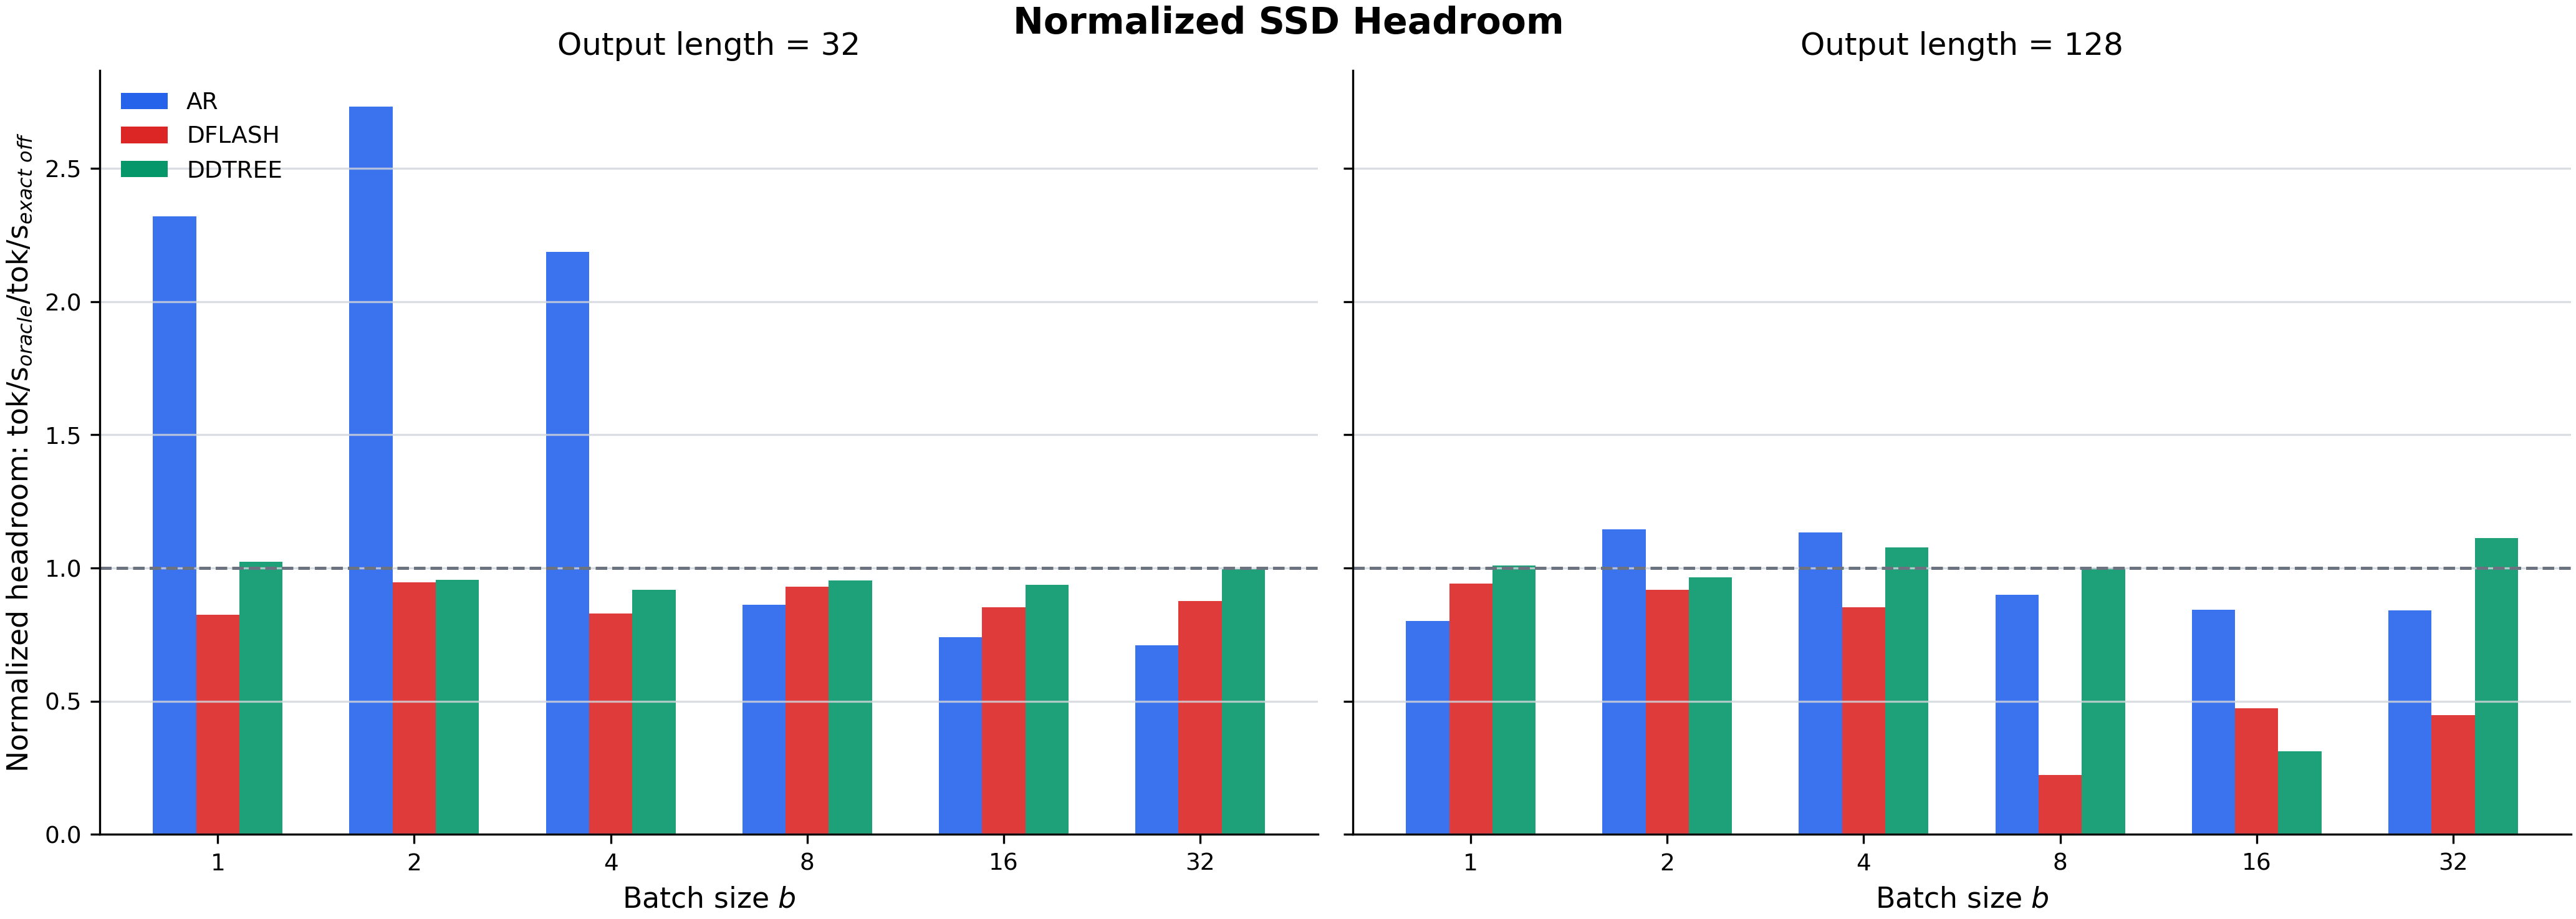
\includegraphics[width=0.96\textwidth]{fig10_normalized_ssd_headroom_b1to32.png}
  \caption{Normalized SSD headroom $=\text{oracle tok/s} \;/\; \text{exact-off tok/s}$ (held constant: Qwen3-8B verifier, greedy decode, fixed branch template; left panel output length~$32$, right panel output length~$128$).
  Values near $1.0$ mean SSD's architectural ceiling offers no meaningful speedup for that family.
  AR has $2.2$--$2.7{\times}$ headroom at $b{\le}4$; both diffusion families hover around $1.0{\times}$, sometimes below.}
  \label{fig:headroom}
\end{figure*}

Figure~\ref{fig:headroom} normalizes by exact-off to remove the per-family throughput baseline.
This view isolates the question \emph{``how much could SSD architecture ever help this family?''}---a question independent of predictor quality.
AR has $2.2$--$2.7{\times}$ headroom in the main regime at $b{\le}4$; DFlash and DDTree hover around $1.0{\times}$.
That gap \emph{is} the negative result: the SSD ``strictly faster than SD'' corollary~\citep{kumar2026ssd} is tight only when the drafter has sequential latency to hide, which diffusion drafters have already spent within a single draft pass.

\subsection{Realized systems: branch-cache failure}
\label{ssec:branchcache}

\begin{figure*}[t]
  \centering
  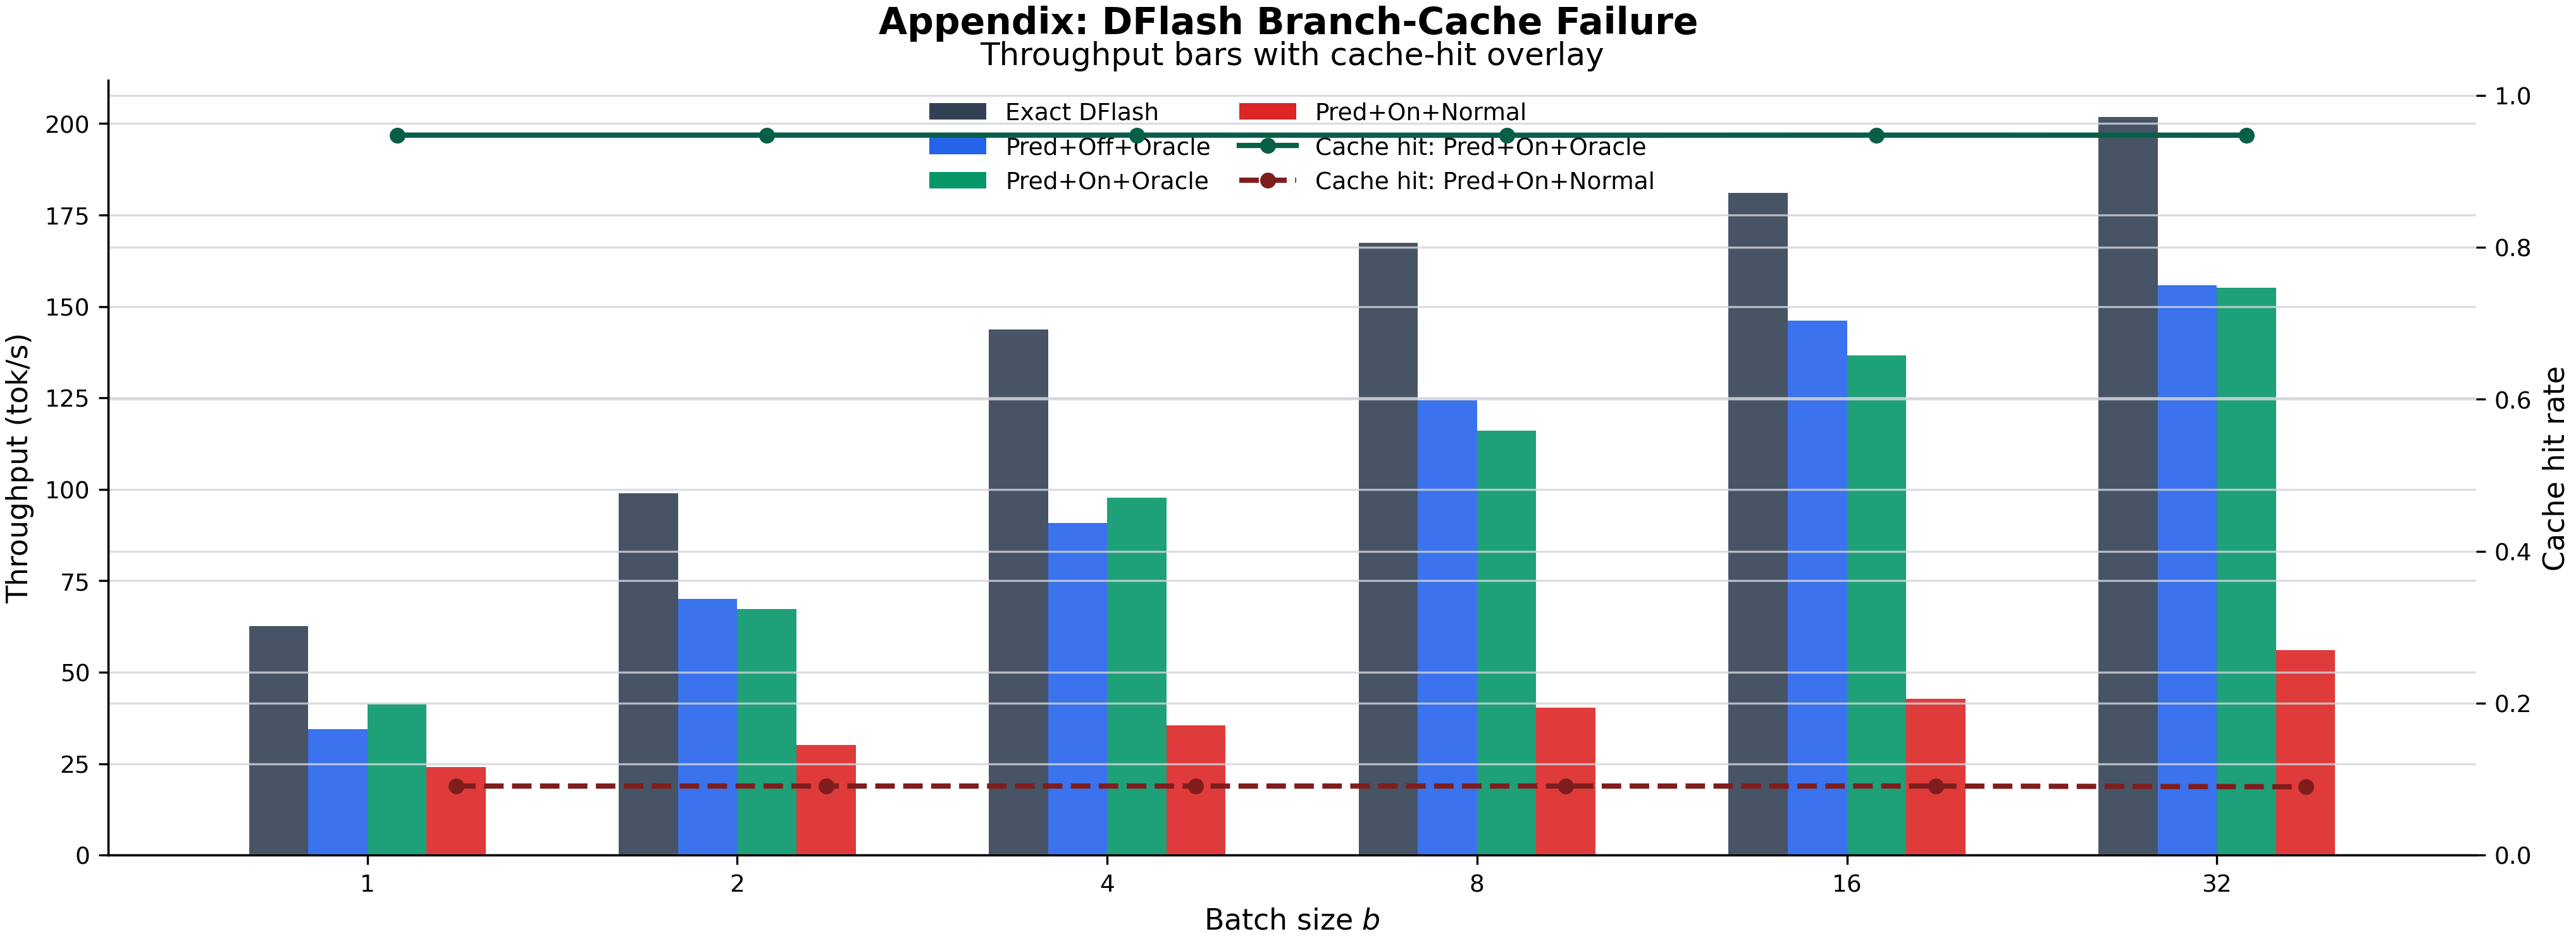
\includegraphics[width=0.96\textwidth]{fig13_dflash_branch_cache_failure_b1to32.png}
  \caption{DFlash branch-cache failure (held constant: Qwen3-8B verifier, output length~$32$, greedy, fixed branch template).
  Bars: throughput under four prediction settings (\textsc{Exact}, \textsc{Pred+Off+Oracle}, \textsc{Pred+On+Oracle}, \textsc{Pred+On+Normal}).
  Lines: the corresponding cache-hit rate.
  Under the realized predictor (\textsc{Pred+On+Normal}, red), the cache-hit rate stays near $0.1$ across all batch sizes, and throughput drops to a fraction of \textsc{Exact}.
  Under an \emph{oracle} predictor (\textsc{Pred+On+Oracle}, green) the hit rate jumps to ${\sim}0.95$ but throughput still does not exceed \textsc{Exact}---confirming that the \emph{architecture}, not just the predictor, is the binding constraint for DFlash.}
  \label{fig:dflash-fail}
\end{figure*}

Figure~\ref{fig:dflash-fail} explains the realized DFlash collapse mechanically.
Even at oracle hit rates ($\sim$$95\%$), DFlash throughput \emph{at no point exceeds the synchronous \textsc{Exact} bar}, again because there is too little serial drafter latency left to hide.
Under the realized predictor, hit rate falls to ${\sim}9\%$, so the realized system pays the worst of both worlds: a wasted pre-draft (because the prediction missed) plus a synchronous fallback draft (full cost).
The corresponding DDTree failure is faster but qualitatively the same: tree budget $N$ controls how many branches are scored in one verifier pass, but the realized hit rate is $<$$1\%$ because the predictor cannot match the diffusion future.

\subsection{$k$-sweep, budget frontier, and long-output regime}
\label{ssec:extra}

A joint sweep over per-family budget knobs ($k\in\{1,2,4,6,8,16\}$ for AR, $(N,F)\in\{8,16\}\times\{1,2\}$ for DDTree, fixed $b{=}16$ block for DFlash) places AR uniformly on the upper-right Pareto front of throughput vs.\ accepted suffix at every $b\in\{1,2,4\}$ (Pareto plot included in the released artifacts).
On the Qwen3-32B cross-check, AR-SSD peaks at $k{=}4$ ($215$~tok/s) and collapses at $k{=}16$ ($103$~tok/s)---the bias-variance-like tradeoff that SSD inherits from SD.
At output length~$128$ (right panel of Figure~\ref{fig:headroom}), DDTree oracle marginally exceeds AR at $b{=}1$ ($128$ vs.\ $106$~tok/s) but AR retakes the lead by $b{=}4$ and the gap widens at $b{\ge}8$; the realized headroom does not translate.

\subsection{Reproducibility}
\label{ssec:repro}
Every number, figure, and table in this report is produced from a single summary artifact emitted by a deterministic wrap-up driver that runs all three drafter families against the same Qwen3-8B verifier with fixed seeds, the same prompt split, and the same branch template, so a re-run regenerates the report end-to-end from one source of truth.
The internal repository documents environment setup, weight download, per-family run drivers, and the figure-rendering step.

%====================================================================
\section{Discussion and Lessons}
\label{sec:disc}

\paragraph{When does SSD help?}
Our evidence converges on one rule: \emph{SSD helps when the drafter has serial latency to hide and the future prefix is cheap to predict}.
AR drafters satisfy both; DFlash satisfies neither (its block is already parallel and its future block is not a simple function of past tokens); DDTree partially satisfies the second via explicit branch uncertainty, which is why its oracle touches AR at $b{=}1$, but the within-round tree already spends most of the parallel budget.

\paragraph{Why can SD/SSD drop \emph{below} target-only AR?}
If SD is exactness-preserving, why does SSD with a $4$B drafter on the Qwen3-32B verifier land at $99$~tok/s---below the target-only baseline ($94$) and below SD ($106$)?
Two effects combine: the drafter and verifier contend for shared GPU compute/KV bandwidth (so the drafter's wall-clock cost is not its FLOP cost), and SSD's scheduler adds per-step overhead (CUDA streams, KV snapshots, the predictor itself, plus a wasted pre-draft on a miss).
When the drafter is large relative to the verifier savings, those overheads flip the inequality---exactly the Qwen3-4B row of Table~\ref{tab:ar-scale} and the same mechanism that pushes realized DFlash below its SD baseline in Table~\ref{tab:main}.
The SSD paper's ``strictly faster than SD'' Corollary~8 assumes zero overhead and $p_{\text{hit}}{>}0$; on a real shared GPU the inequality is not safe to invoke.

\paragraph{What the negative result is \emph{not}.}
Diffusion drafters are not useless under standard SD: DFlash and DDTree both clear AR at every batch size in our main regime ($62.5/82.0$ vs.\ $40.1$ at $b{=}1$, Table~\ref{tab:main}), and DDTree is the best family in our long-output regime.
We only claim that \emph{grafting SSD onto them does not unlock additional throughput}.

\paragraph{Limitations.}
One verifier (Qwen3-8B), one dataset family (GSM8K-style), $2{\times}$H100 hardware; our DFlash predictor saw mode collapse, but a better predictor cannot lift the \emph{oracle} ceiling itself---which is where the diffusion story is lost.

\paragraph{Future work.}
Two directions: \emph{hybrid drafters} that put a tiny AR head on top of a DFlash block to re-introduce serial latency for SSD to hide; and \emph{predictor fusion} into the verifier's last layer (à la EAGLE~\citep{li2024eagle}) to amortize predictor cost into the same forward pass and remove the scheduling overhead that flips the SSD inequality for fat drafters.

%====================================================================
\section{Team Contributions}
\label{sec:contrib}
All three authors worked jointly on project scope and writing.
\textbf{Aditya Ramesh} led the tree-diffusion side: integrating DDTree~\citep{ringel2026ddtree} into the async runtime, sweeping its tree-budget/frontier knobs $(N,F)$, and positioning the project against TiDAR and ``Your LLM Knows the Future''.
\textbf{Arav Tewari} led the diffusion side of the stack: integrating DFlash into the async runtime, training the DFlash predictor, and diagnosing the mode-collapse failure.
\textbf{Xinyu Jiang} led the experimental pipeline: AR baselines under SD/SSD across batch sizes and drafter scales, the oracle/exact-off/realized decomposition, figures, tables, and drafting this report.

%====================================================================
\section{Conclusion}
\label{sec:conc}
We tested whether diffusion drafters---which parallelize \emph{within} a draft step---are better SSD partners than AR drafters.
Under a matched-budget evaluation on Qwen3-8B with three drafter families and three modes, the answer is no at every batch size in our main regime; the explanation is mechanical, that SSD's overlap has room only when drafter latency is serial, which diffusion has already spent within a single block.
Future diffusion-SSD hybrids must first demonstrate non-trivial \emph{oracle} headroom before investing in realized-system engineering.

\section*{Acknowledgements}
We thank the 18-789 course staff for compute and guidance, and the authors of the SSD, DFlash, and block-diffusion papers for releasing code and checkpoints.

\bibliography{final_report}
\bibliographystyle{reportstyle}

\end{document}
